\documentclass[11pt, a4paper]{article}
\usepackage[a4paper, margin = 0.7in]{geometry}
\usepackage{graphicx}
\usepackage{amsmath}
\usepackage{listings}
\usepackage{url}

\title{EE2703 Assignment 6B : The Laplace Transform}
\author{Aman Kumar EE19B066}
\date{April 26, 2021}

\begin{document}

\maketitle

\section{The Assignment}
In this assignment, we looked at how to analyse “Linear Time-invariant Systems”
with the \textit{signal toolbox} in Python. We have considered three systems in this assignment:
\begin{itemize}
    \item A forced oscillatory system.
    \item A coupled system of Differential Equations.
    \item A low pass  RLC filter.
\end{itemize}

\section{Assignment questions}
\subsection{Question 1}
    Here we have to solve for the time response of a spring satisfying:
    \begin{equation*}
        \ddot x + 2.25x = f(t)
    \end{equation*}
    where $x(0) = 0 = \dot x(0)$. Here $f(t) = cos(1.5t)e^{-0.5t}u_0(t)$ and its Laplace transform is gicen by:
    \begin{equation*}
        F(s) = \frac{s + 0.5}{(s + 0.5)^2 + 2.25}
    \end{equation*}
    So, solving for $X(s)$ we get
    \begin{equation}
        X(s) = \frac{F(s)}{s^2 + 2.25}
    \end{equation}
    So, to get $x(t)$ we find its impulse response and plot it for $t = 0$ to $t = 50$ seconds
    \begin{figure}[!h]
        \centering
        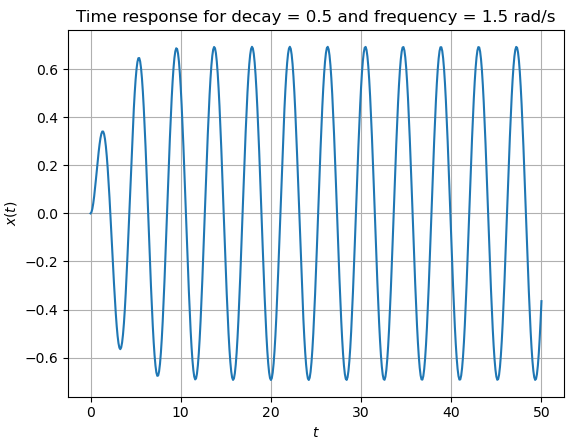
\includegraphics[scale = 0.62]{Figure 1.png}
        \caption{Time response with decay = 0.5}
        \label{fig:Figure 1}
    \end{figure}

The python code snippet(some unimportant parts omitted) for this-
    \begin{verbatim}
def spring_Trnsfr(decay,freq):
    return(sp.lti([1,decay],[1,2*decay,decay**2 + freq**2 + 2.25,4.5*decay,
           2.25*(decay**2 + freq**2)]))
           
X1 = spring_Trnsfr(0.5,1.5)       #Transfer function with decay = 0.5, freq = 1.5
t,x = sp.impulse(X1,None,pl.linspace(0,50,501))

#Plotting x(t)
pl.figure(0)
pl.plot(t,x,label="$x(t)$")
    \end{verbatim}

\subsection{Question 2}
Doing the same thing but with a much smaller decay. This time decay = $0.05$
    \begin{verbatim}
X2 = spring_Trnsfr(0.05,1.5)      #Transfer function with decay = 0.05, freq = 1.5
t,x = sp.impulse(X2,None,pl.linspace(0,50,501))
    \end{verbatim}
    \begin{figure}[!h]
        \centering
        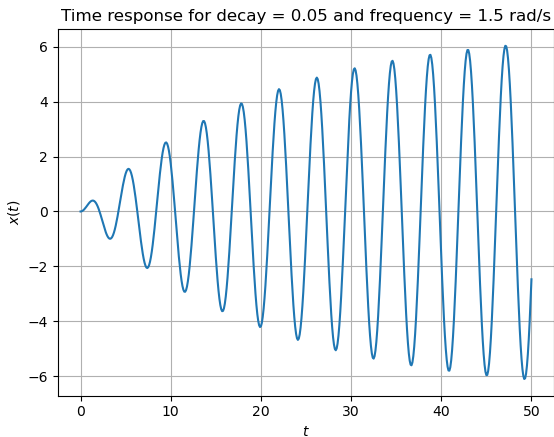
\includegraphics[scale = 0.8]{Figure 2.png}
        \caption{Time response with decay = 0.05}
        \label{fig:Figure 2}
    \end{figure}
    
    We can see that the result is very similar to that of question 1, except with a diferent amplitude. This is because the system takes longer to reach a steady state.
    
\subsection{Question 3}
    Now we try to see what happens when we vary the frequency of the forcing function $f(t)$. We vary the frequency from $1.4$ to $1.6$ in steps of $0.05$ while keeping decay as $0.05$. We notice that the amplitude is maximum for $f = 1.5$ which is also the natural frequency of the system. Thus it shows resonance:
    \begin{verbatim}
Freq = pl.arange(1.4,1.65,0.05)           #Frequency vector 1.4 to 1.6 rad/s
H = sp.lti([1],[1,0,2.25])                #The transfer function 1/(s^2 + 2.25)
t = pl.linspace(0,100,1001)               #Simulating for 100 s
label_ = []                               #For making the legend                

pl.figure(2)
pl.title("Time response of spring with different frequency inputs")
pl.xlabel("$t$")
pl.ylabel("$x(t)$")

for fq in Freq:
    f = pl.cos(fq*t)*pl.exp(-0.05*t)*(t>0)   #Input function
    t,x,svec = sp.lsim(H,f,t)
    pl.plot(t,x)      #Plotting time response on the same plot for all frequencies
    label_.append("f = "+ str(fq))
    
pl.legend(label_)
pl.show()
    \end{verbatim}
    \begin{figure}[!h]
        \centering
        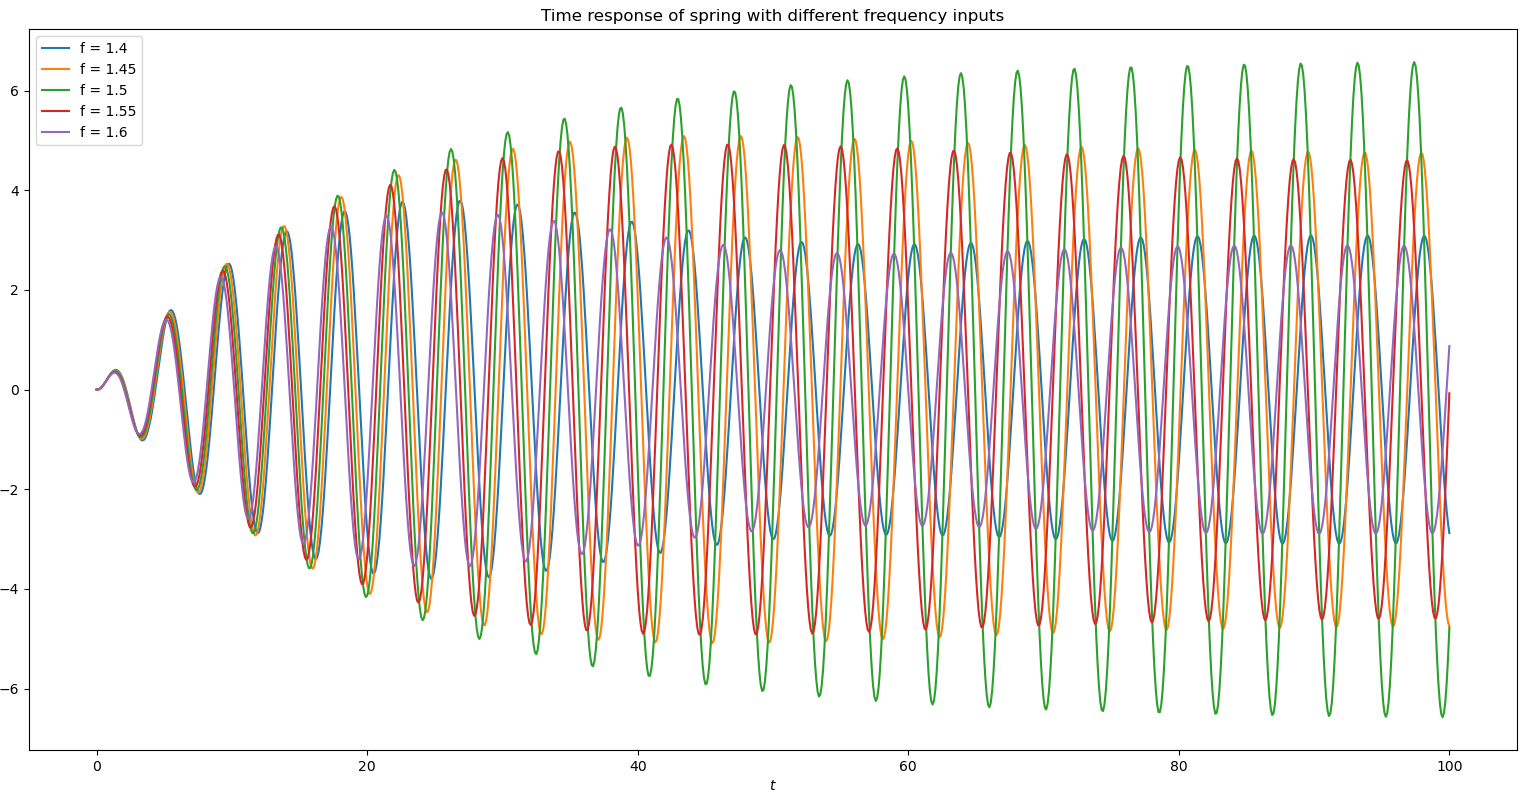
\includegraphics[scale = 0.44]{Figure 3.png}
        \caption{Time response with frequency varying from 1.4 to 1.6 rad/s}
        \label{fig:Figure 3}
    \end{figure}
    
\subsection{Question 4}
    We have to now solve for the coupled spring problem:
    \begin{equation*}
        \ddot x + (x - y) = 0
    \end{equation*}
    \begin{equation*}
        \ddot y + 2(x - y) = 0
    \end{equation*}
    with $x(0) = 1$, $\dot x(0) = y(0) = \dot y(0)$. Solving we get:
    \begin{equation}
        X(s) = \frac{s^2 + 2}{s^3 + 3s}
    \end{equation}
    \begin{equation}
        Y(s) = \frac{2}{s^3 + 3s}
    \end{equation}
    Thus we find $x(t)$ and $y(t)$ using \textit{scipy.signal.impulse}, and plot them on same plot for $t = 0$ to $t = 20$ seconds.
    \begin{verbatim}
X = sp.lti([1,0,2],[1,0,3,0])                     #X(s) = (s^2 + 2)/(s^3 + 3s)
Y = sp.lti([2],[1,0,3,0])                         #Y(s) = 2/(s^3 + 3s)

t,x = sp.impulse(X,None,pl.linspace(0,20,201))    #Finding x(t)
t,y = sp.impulse(Y,None,pl.linspace(0,20,201))    #Finding y(t)
    \end{verbatim}
    \begin{figure}[!h]
        \centering
        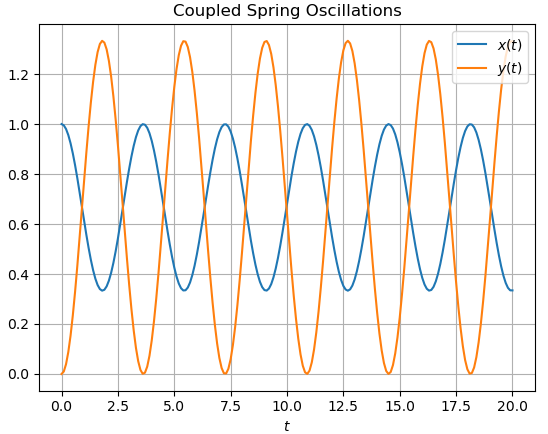
\includegraphics[scale = 0.8]{Figure 4.png}
        \caption{Coupled spring system}
        \label{fig:Figure 4}
    \end{figure}
    
\subsection{Question 5}
    In this question w have to plot the magnitude and phase response of the transfer function of a given RLC circuit. It is an RLC, second order low pass filter. The transfer function is:
    \begin{equation}
        H(s) = \frac{1}{s^2LC + sCR + 1}
    \end{equation}
    \begin{verbatim}
H = sp.lti([1],[1e-12,1e-4,1])          #Defining the system transfer function
w,S,phi = H.bode()

pl.figure(4)
pl.subplot(2,1,1)                       #First subplot is for Magnitude response
pl.title("Magnitude response")
pl.xlabel("$w$")
pl.ylabel("|H(jw)| (dB)")
pl.semilogx(w,S)
pl.grid(True)
pl.subplot(2,1,2)                       #Second subplot is for Phase response
pl.title("Phase Response")
pl.semilogx(w,phi)
pl.xlabel("$w$")
pl.ylabel("phase(H(jw)) (degrees)")
pl.semilogx(w,phi)
pl.grid(True)
pl.show()
    \end{verbatim}
    \begin{figure}[!h]
        \centering
        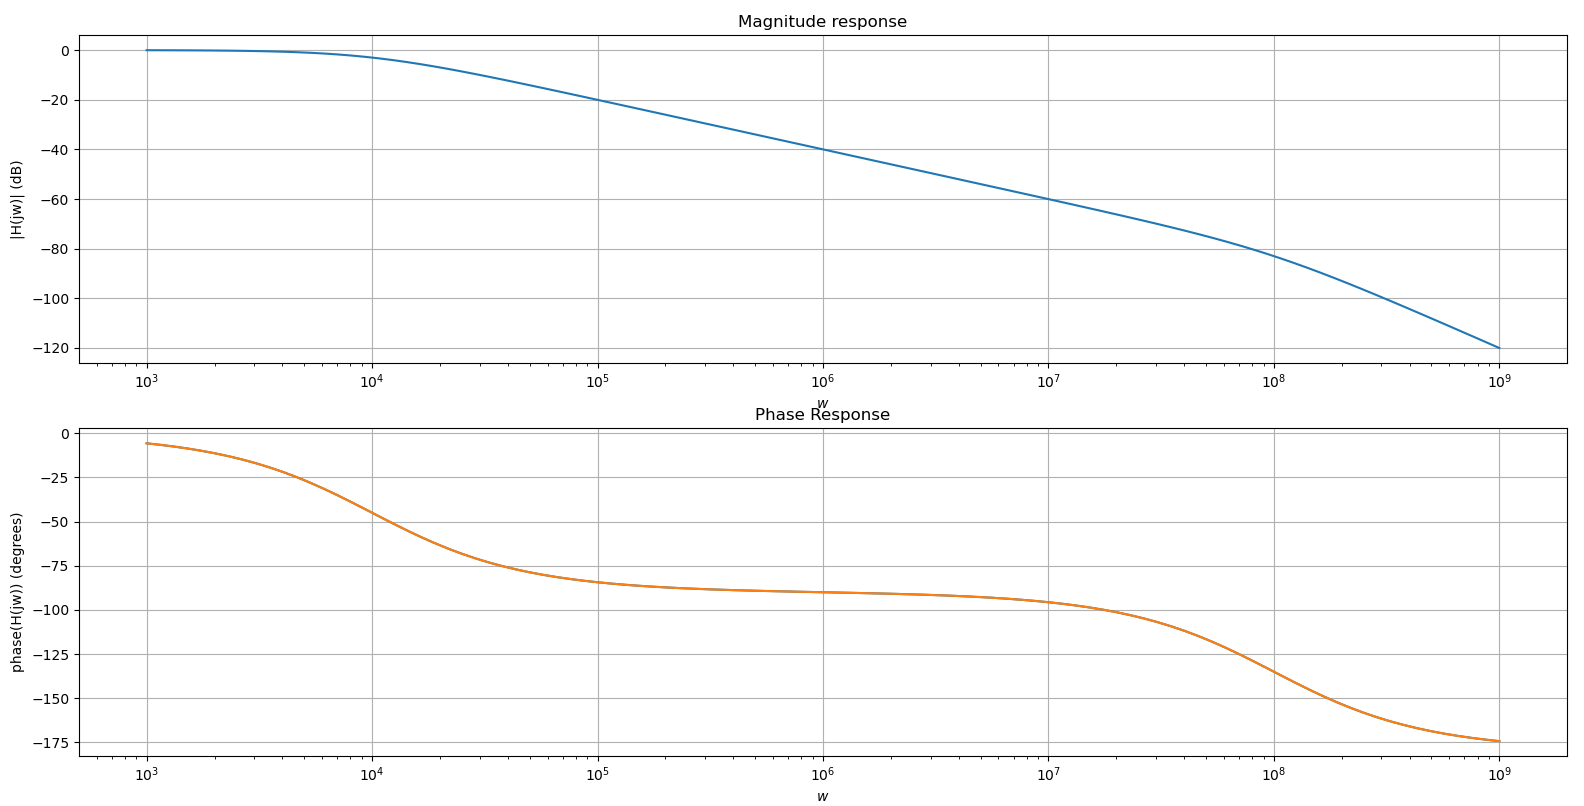
\includegraphics[scale = 0.43]{Figure 5.png}
        \caption{Bode Plot of the RLC circuit}
        \label{fig:Figure 5}
    \end{figure}

\subsection{Question 6}
    In this question we have to plot the response($v_o(t)$) the given RLC circuit to input voltage $v_i(t)$ given by:
    \begin{equation*}
        v_i(t) = cos(10^3t)u(t) - cos(10^6t)u(t)
    \end{equation*}
    \begin{verbatim}
t = pl.arange(0,0.01,1e-7)                   #time vector from 0 to 10ms
Vin = (pl.cos(1e3*t) - pl.cos(1e6*t))*(t>0)  #Input voltage vector
t,Vout,svec = sp.lsim(H,Vin,t)               #Finding the output voltage vector
    \end{verbatim}
    \begin{figure}[!h]
        \centering
        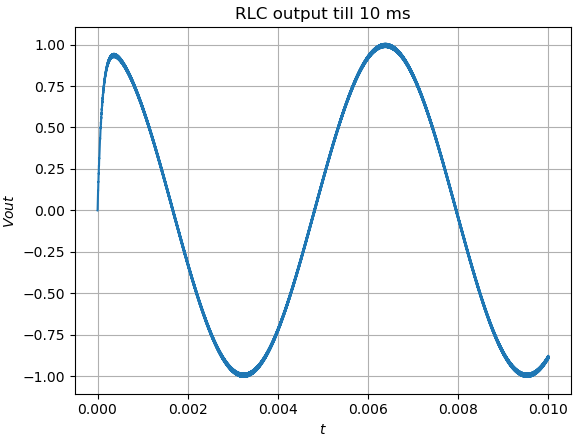
\includegraphics[scale = 0.65]{Figure 6.png}
        \caption{$v_o(t)$ till 10 ms}
        \label{fig:Figure 6}
    \end{figure}
    \begin{verbatim}
#Plotting output voltage from 0 to 10ms
pl.figure(5)
pl.title("RLC output till 10 ms")
pl.plot(t,Vout)

#Plotting output voltage from 0 to 30us
pl.figure(6)
pl.title("RLC output till 30 us")
pl.plot(t[:301],Vout[:301])
    \end{verbatim}
    \begin{figure}[!h]
        \centering
        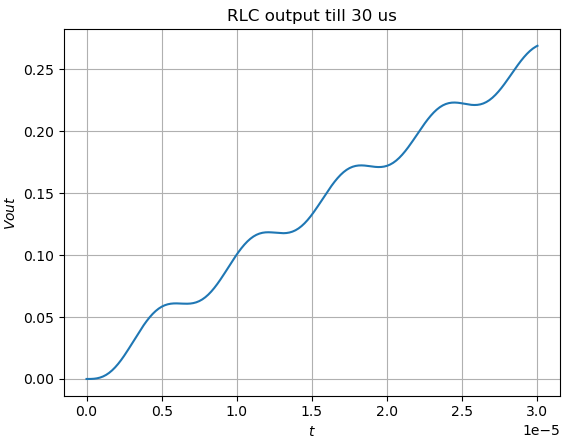
\includegraphics[scale = 0.7]{Figure 7.png}
        \caption{$v_o(t)$ till 30 $\mu s$}
        \label{fig:my_label}
    \end{figure}

\section{Conclusion}
In this assignment we learnt how to use the \textit{signal toolbox} to work with LTI systems.This is very helpful as LTI systems are observed in all fiels of engineering and are very important. We learnt to find impulse response, we learnt to use transfer function to find the output if input is given.
\end{document}
